\documentclass{article}
\usepackage[utf8]{inputenc}
\usepackage[T2A]{fontenc}
\usepackage[russian]{babel}
\usepackage[left=30mm,right=10mm]{geometry}


\begin{center}
    \textbf{\huge {Использование искусственного интеллекта в торговле: проблемы и перспективы}}\\
    \vspace{5mm}
   \textbf{\large{Аннотация}} 
\end{center}

Рассмотрены важные аспекты применения искусственного интеллекта в торговле, выявлены ключевые преимущества и недостатки, проанализированы современные тренды и перспективы развития в области искусственного интеллекта.
\vspace{5mm}
\newline{\textbf{Ключевые слова:} искусственный интеллект, торговля, автоматизация, прогнозирование, эффективность.}


\section*{\hspace{10mm}Введение}
\normalsize{\hspace{5mm}Искусственный интеллект (ИИ) в последние годы активно проникает в различные сферы деятельности и человеческую жизнь. Одной из наиболее динамично развивающихся областей его применения стала торговля. Ритейлеры и бренды по всему миру быстро внедряют технологии искусственного интеллекта. Всемирно известная американская компания по производству одежды "Levi's", которая использует ИИ для генерации моделей людей. Магазин одежды ThredUp – чтобы запомнить предпочтения клиентов, или Amazon, которая заменила кассиров при помощи ИИ. Можно сказать, что искусственный интеллект дает много перспективных и современных возможностей, которые очень сильно упрощают работу людей в сфере торговли.}

\section*{\hspace{10mm}Возможности внедрения ИИ в торговле}
\normalsize{\hspace{5mm}Искусственный интеллект имеет огромное количество возможностей использования в сфере торговли, помогающие не только в торговой деятельности, но и покупателям совершать покупки, поэтому будет целесообразно разделить данную тему на несколько подразделов.}

\section{Снижение расходов}
\normalsize{\hspace{5mm}ИИ снижает количество расходов за счет сокращения рабочих мест при внедрении чат-бота с ИИ и замены штата операторов [1, с. 252].}
\section{Повышение эффективности торговли}
\normalsize{\hspace{5mm}Искусственный интеллект изучает большие объемы информации и выдвигает гипотезы для персонализации контента быстрее и точнее, чем человек.}
\section{Анализ неструктурированных данных}
\normalsize{\hspace{5mm}В последнее время в ИИ используются все более крупные наборы данных, для прогнозирования финансово-экономических процессов торговли. При невозможности организации заранее заданной структуры данных, ИИ позволяет структурировать и анализировать их. По оценке Mapp, ведущего поставщика услуг по обслуживанию клиентов, основанных на аналитике, на 2019 год около 90\% всех генерируемых данных не структурированы, а, следовательно, большая часть оставалась ранее неиспользованной [2, с. 173-174].}
\section{Прогнозирование цен с помощью ИИ}
\normalsize{\hspace{5mm}До внедрения ИИ не было возможности предугадать товарные предпочтения клиентов. Единственное, что делали ритейлеры, – интуитивно предсказывали, в какой момент времени можно будет поднять цены на определенные товары, пользующиеся спросом потребителей. Благодаря возможностям искусственного интеллекта ритейлерам предоставляется возможность прогнозировать предпочтения клиентов и уровень повышения цен, при которой товары будут пользоваться спросом.

При прогнозировании необходимо проводить большую работу с огромным объемом данных. С помощью систем ИИ можно оперативно, мгновенно анализировать всю доступную информацию, данные, появляющиеся каждую секунду, сравнивая и анализируя их с более ранней информацией, выявляя конкурентов, тенденции и изменения в покупательском поведении, получая точный прогноз о том, какая цена устроит покупателей в определенный момент времени [2, c. 173-174] [3].}
\section{Оптимизация цен}
\normalsize{\hspace{5mm}После получения всей информации о наиболее подходящей цене, ритейлерам остается придумать стратегию оптимизации цен и сделав ее максимально сбалансированной, отвечающей конъюнктуре рынка. Стратегия должна учитывать с одной стороны, возможность получения максимальной прибыли для компании, с другой – уложиться в ожидания клиентов относительно цен. На этих направлениях начинается самое перспективное применение ИИ в ритейле.

Согласно исследованию Ассоциации электронных коммуникаций (РАЭК), 42\% крупнейших российских ритейлеров («Пятерочка», «Перекресток», «Чижик») в настоящее время используют технологии и решения на основе искусственного интеллекта, а еще 35\% – планируют начать использовать в течение 5 лет. В ближайшее пятилетие технологии и решения на основе искусственного интеллекта будет использовать 77\% российских ритейлеров [4, c. 7].}
\section{Маркетинг}
\normalsize{\hspace{5mm}Особое место искусственный интеллект занимает в маркетинге. Благодаря синтезу технологий глубинного обучения, машинного зрения и когнитивной нейробиологии искусственный интеллект может быть применен как для исследования рынка, так и для персонализации контента с целью улучшения процесса анализа информации и определения масштаба воздействия на потребителей без лишних затрат.

Среди основных направлений применения искусственного интеллекта в маркетинге выделяют веб-дизайн, контекстную рекламу, оценку эффективности проведенных рекламных кампаний, поиск по фотографиям, получение сведений рекламодателям для предоставления новостей или рекламной информации.

Одно из наиболее перспективных направлений применения искусственного интеллекта в сфере маркетинга – это возможность персонализировать рекламный контент, давая каждому потребителю подходящие именно для него предложения. Правильное сообщение будет приходить нужному человеку в нужное время [5, с. 80].}

\section{Управление складом}
\normalsize{\hspace{5mm}Одним из видов искусственного интеллекта, являются голосовые ассистенты. Система голосового управления на базе технологии системы Voice позволяет, сократить время сборки заказов, снизить количество ошибок при комплектовании заказа, уменьшить количество бумажной документации на складе, повысить эффективность складского персонала, оперативно отслеживать ошибки инвентаризации, а также увеличить производительность и пропускную способность склада.

В данный момент при использовании технологии искусственного интеллекта возможности программного продукта существенно расширились. Сейчас система может не только указывать расположение товара на складе, но и подсказывать/формировать наиболее оптимальный путь до расположения ячейки и впоследствии наиболее удачно размещать его исходя из востребованности и товарного соседства, при этом учитывая многие другие факторы, такие как температура, освещенность, сроки годности. Так же система ИИ анализирует входящую информацию по приходам товара и отгрузкам, выявляет непрогнозируемые пики, помогая руководителям распределительных центров самостоятельно грамотно распределять персонал [6, с. 33-34].}

\section*{\hspace{10mm}Характеристика систем ИИ в торговле}
\normalsize{\hspace{5mm}ИИ анализирует сведения о конкретном ритейлере и его бизнес-процессах. Система оценивает количество товаров на складе, анализирует самые продаваемые товары, учится понимать, в какой момент времени какие товары реализовать лучше всего и по какой цене. Он также определяет, как скидка на один товар повлияет на продажи другого, и предлагает наиболее оптимальную стратегию, при которой покупатель обязательно купит, а продавец обязательно получит прибыль. 60\% покупателей выбирают предложения с оптимальным соотношением “цена-качество”, хотя, конечно, анализ потребительского поведения показывает, что важны и другие факторы.}
\section*{\hspace{10mm}Перспективы развития ИИ}
\normalsize{\hspace{5mm}Согласно исследованию корпорации IBM, ожидается, что внедрение искусственного интеллекта в розничной торговле потребительскими товарами вырастет с 40\% компаний в настоящее время до более чем 80\% через три года [7] в счет увеличения инвестиций розничной торговли в технологии ИИ. За это время инвестиции в прогнозную и предписывающую аналитику на основе искусственного интеллекта удвоятся.

Объем глобального искусственного интеллекта на розничном рынке оценивается в 5,50 млрд долларов в 2022 году и, по прогнозам, вырастет с 7,14 млрд долларов в 2023 году до 55,53 млрд долларов к 2030 году, демонстрируя среднегодовой темп роста 34,1\%, в течение прогнозируемого периода.}
\section*{\hspace{10mm}Развитие торговли в Республике Беларусь}
\normalsize{\hspace{5mm}В кризисные 90е годы торговля являлась единственной развивающейся отраслью экономики, благодаря которой высвобождающиеся работники, крупных валообразующих предприятий смогли получать доход, осуществляя челночную торговлю. Основные экономические показатели, розничный товарооборот, количество предприятий и количество работников торговли, за последнее десятилетие приведены в таблице 1, рисунках 1, 2 и 3.}

\begin{table}[t]
    \begin{tabular}{||p{0.5\textwidth}|c|c|c|c|c||}
    \hline Показатель & 2010 & 2015 & 2020 & 2021 & 2022 \\
    \hline  
    Розничный товарооборот, млн руб. & 6486,5 & 34724 & 53539 & 60067 & 68059\\
    \hline 
    Количество предприятий & 43754 & 46228 & 41123 & 39913 & 39780 \\
    \hline 
    Количество работников, тыс. & 625,7 & 650,6 & 620 & 609,2 & 600,6 \\
    \hline 
    \end{tabular}
    \bfseries\caption{Основные экономические показатели розничной торговли}
\end{table}

\begin{figure}
    \centering
    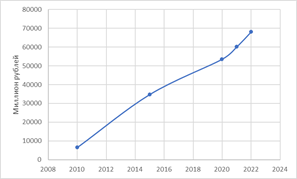
\includegraphics[width=0.45\linewidth]{image1.png}
    \caption{Розничный товарооборот за 2010-2022 годы}
\end{figure}
\begin{figure}
    \centering
    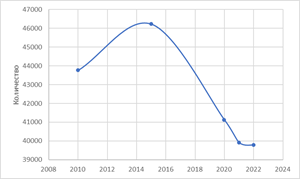
\includegraphics[width=0.45\linewidth]{image2.png}
    \caption{Количество предприятий за 2010-2022 годы}
\end{figure}
\begin{figure}
    \centering
    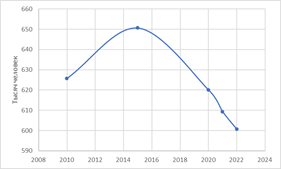
\includegraphics[width=0.45\linewidth]{image3.png}
    \caption{Количество работников торговли за 2010-2022 годы}
\end{figure}

Число работников увеличивалось быстрым темпом до 2015 года, затем прослеживаются сокращения на 7,68\%. Количество предприятий также сократилось с 43 тысяч, в 2010 году, до 39 тысяч в 2022 году, за счет ухода с рынка малых и средних предприятий и приходящих отечественных и зарубежных сетей. Розничный товарооборот неуклонно растет с 2010 года, что свидетельствует о повышении качества жизни.

\section*{\hspace{10mm}Недостатки внедрения ИИ в торговлю}
\normalsize{\hspace{5mm}К недостаткам ИИ относятся: безопасность данных, необходимость кадровых ресурсов с экспертизой в области ИИ и этические вопросы. Так же ИИ не умеет рисковать, хотя риск бывает оправдан. Он принимает основанные на логике решения, исходя из данных. Такие решения не всегда оказываются выгодными и правильными, однако количество ошибок, в сравнении с человеком значительно меньше [6, c. 26].

Решение этих проблем требует комплексного подхода и сотрудничества между бизнесом, научным сообществом и правительством.}

\section*{\hspace{10mm}Выводы}
\normalsize{\hspace{5mm}Искусственный интеллект демонстрирует свою важную роль в торговле, эффективно изменяя ландшафт бизнеса. В условиях возрастающей конкуренции ИИ становится неотъемлемым партнером для компаний, стремящихся оставаться конкурентоспособными и реагировать на потребности современных клиентов. Как было показано ИИ имеет как целый ряд возможностей и преимуществ, так и некоторые недостатки, и потенциальные проблемы.  ИИ несомненно остается ключевым фактором успеха для компаний, в быстро меняющемся мире торговли.}

\section*{\hspace{10mm}Список литературы}

\begin{enumerate}
\item Тихоновская, Ю.О., Федечко, А.А. Искусственный интеллект и маркетинг [Электронный ресурс] // Пинск 2023.— Режим доступа: URL: https://rep.polessu.by/handle/123456789/29347 (дата обращения 03.12.2023)
\item Тавлуй Д. В., Алексеев В. Ф., Пискун Г. А. Использование искусственного интеллекта в интернет-маркетинге. – 2023 – 6 c.
\item How AI Can Help the Retail Industry with Price Prediction and Price Optimization [Электронный ресурс]. – Режим доступа: URL: https://semupdates.com/how-ai-can-help-the-retail-industry-with-price-prediction-and-price-optimization/ (дата обращения 09.10.2023)
\item Искусственный интеллект для маркетинга [Электронный ресурс]. – Режим доступа: URL: https://raec.ru/ii-retail-2020.pdf. (дата обращения 26.11.2023)
\item Калиновская И. Н., Шерстнева О. М. Интеграция искусственного интеллекта в маркетинг. – 2018 – 4 c.
\end{enumerate}

\end{document}
